\documentclass[10pt,a4paper]{article}
\usepackage[T1]{fontenc}
\usepackage[utf8]{inputenc}
\usepackage{charter}
\usepackage[scaled=0.92]{helvet}
\usepackage{amsmath}
\usepackage[margin=1cm,top=1.5cm,bottom=1.5cm]{geometry}
\usepackage{microtype}
\usepackage{xcolor}
\usepackage{graphicx}
\usepackage{float}
\usepackage{needspace}
\usepackage{booktabs,array,tabularx}
\usepackage{titlesec}
\usepackage{fancyhdr}
\usepackage{enumitem}
\usepackage{caption}
\usepackage{subcaption}
\usepackage{listings}
\usepackage{tikz}
\usetikzlibrary{positioning,arrows.meta,calc,fit,backgrounds,shapes.geometric}
\usepackage[most]{tcolorbox}
\usepackage[colorlinks=true,linkcolor=teal,urlcolor=teal,citecolor=teal]{hyperref}

% auto-generated by make_assets.py - do not edit
\newcommand{\xNTrain}{48{,}000}
\newcommand{\xNVal}{12{,}000}
\newcommand{\xNegWeightTrain}{292}
\newcommand{\xNegWeightVal}{145}
\newcommand{\xMissWeightTrain}{300}
\newcommand{\xMissWeightVal}{165}
\newcommand{\xMissMITrain}{374}
\newcommand{\xMissMIVal}{249}
\newcommand{\xNUnseen}{8}
\newcommand{\xUnseenRows}{1{,}447}
\newcommand{\xUnseenList}{Allentown, Charlotte, Chicago, Jackson, Knoxville, Laredo, Norfolk, San Diego}
\newcommand{\xMIWithinStd}{0.025}
\newcommand{\xMITrainMin}{0.68}
\newcommand{\xMITrainMax}{1.47}
\newcommand{\xMIValMin}{0.72}
\newcommand{\xMIValMax}{1.10}
\newcommand{\xMIValMean}{0.93}
\newcommand{\xDistFloor}{70}
\newcommand{\xNCities}{64}
\newcommand{\xElastDist}{0.87}
\newcommand{\xReeferPct}{13}
\newcommand{\xFlatbedPct}{8}
\newcommand{\xCoreSigma}{4.0}
\newcommand{\xSpikePct}{1.4}
\newcommand{\xSpikeHiMult}{2.2--5.4}
\newcommand{\xSpikeLoMult}{0.17--0.45}
\newcommand{\xOffset}{+1.3\%}
\newcommand{\xGainMAE}{14}
\newcommand{\xGainMed}{37}
\newcommand{\xFinalMAE}{119.4}
\newcommand{\xFinalMed}{2.16}
\newcommand{\xFinalMAPE}{5.20}
\newcommand{\xOffsetGainMAE}{7.0}
\newcommand{\xTopFeature}{log distance}
\newcommand{\xMedAPEFold}{2.07}
\newcommand{\xMedAPEShort}{2.2}
\newcommand{\xMedAPELong}{1.7}
\newcommand{\xDecMin}{805}
\newcommand{\xDecMax}{813}
\newcommand{\xDecMean}{808}
\newcommand{\xDecSpreadPct}{0.9}


% ---------- editable ----------
\newcommand{\reportauthor}{Azizul Abedin Azmi}
\newcommand{\repourl}{github.com/azizulabedinazmi/freight-rate-ml}
% ------------------------------

\definecolor{teal}{HTML}{064A56}
\definecolor{mid}{HTML}{2A9D8F}
\definecolor{lightteal}{HTML}{E8F2F3}
\definecolor{coral}{HTML}{E4572E}
\definecolor{ink}{HTML}{25363A}
\definecolor{greyline}{HTML}{BFD0D3}

\newcommand{\sans}{\fontfamily{phv}\selectfont}
\titleformat{\section}{\sans\Large\bfseries\color{teal}}{\thesection}{0.6em}{}[{\color{greyline}\titlerule[0.6pt]}]
\titleformat{\subsection}{\sans\large\bfseries\color{teal}}{\thesubsection}{0.6em}{}
\titlespacing*{\section}{0pt}{16pt}{8pt}
\titlespacing*{\subsection}{0pt}{11pt}{4pt}
\captionsetup{font={small,sf},labelfont={bf,color=teal},labelsep=period,skip=5pt}
\setlist{itemsep=2pt,topsep=3pt,leftmargin=1.3em}
\renewcommand{\arraystretch}{1.18}
\setlength{\parskip}{4pt}\setlength{\parindent}{0pt}

\pagestyle{fancy}\fancyhf{}
\renewcommand{\headrulewidth}{0pt}
\fancyhead[L]{\sans\scriptsize\color{teal}\textbf{Freight Rate Prediction}\ \textcolor{ink}{$\cdot$ ML Engineer Assessment}}
\fancyhead[R]{\sans\scriptsize\color{ink}\reportauthor}
\fancyfoot[C]{\sans\scriptsize\color{ink}\thepage}

\lstdefinestyle{py}{basicstyle=\ttfamily\footnotesize\color{ink},keywordstyle=\color{teal}\bfseries,
  commentstyle=\color{mid}\itshape,stringstyle=\color{coral},language=Python,columns=fixed,
  keepspaces=true,showstringspaces=false,breaklines=true,frame=none,xleftmargin=0pt,aboveskip=0pt,belowskip=0pt}
\newtcolorbox{callout}[1][]{enhanced,breakable,colback=lightteal,colframe=lightteal,
  borderline west={2.5pt}{0pt}{teal},sharp corners,left=9pt,right=8pt,top=5pt,bottom=5pt,
  fonttitle=\sans\bfseries\color{teal},#1}
\newtcolorbox{codebox}{enhanced,colback=white,colframe=greyline,boxrule=0.5pt,arc=2pt,left=6pt,right=6pt,top=4pt,bottom=4pt}

\newcommand{\stat}[3]{%
  \begin{tcolorbox}[enhanced,colback=white,colframe=greyline,boxrule=0.6pt,arc=3pt,width=\linewidth,
    left=2pt,right=2pt,top=1pt,bottom=4pt,halign=center]
    {\sans\fontsize{20}{22}\selectfont\bfseries\color{#3}#1}\\[1pt]
    {\sans\scriptsize\color{ink}#2}
  \end{tcolorbox}}

\begin{document}

% ================= TITLE BLOCK =================
\noindent

\begin{tikzpicture}
  \fill[teal] (0,0) rectangle (\textwidth,3.5);
  \fill[mid] (0,0) rectangle (0.28,3.5);
  \fill[white,opacity=0.07] (\textwidth,3.5) arc (90:180:5.2) -- (\textwidth,0) -- cycle;
  \node[anchor=west,text=white,align=left] at (0.8,2.45)
    {\sans\fontsize{23}{26}\selectfont\bfseries Freight Rate Prediction};
  \node[anchor=west,text=white,align=left] at (0.8,1.65)
    {\sans\large Validation approach, data quality, and the December forecast};
  \node[anchor=west,text=white!80,align=left] at (0.8,0.7)
    {\sans\small Machine Learning Engineer assessment \quad$\cdot$\quad \reportauthor \quad$\cdot$\quad \texttt{\repourl}};
\end{tikzpicture}
\par\vspace{-\parskip}
\noindent
\begin{minipage}{0.31\textwidth}\stat{\$\xFinalMAE}{mean abs. error, forward-in-time CV}{teal}\end{minipage}\hfill
\begin{minipage}{0.31\textwidth}\stat{\xFinalMed\%}{median abs.\ \% error}{mid}\end{minipage}\hfill
\begin{minipage}{0.31\textwidth}\stat{$-\xGainMAE$\%}{MAE vs.\ linear baseline}{coral}\end{minipage}


\begin{callout}[title=Summary]
The task is to price \xNVal{} loads from November--December 2025 using \xNTrain{} labelled loads from January--October.
Because the targets lie in the \emph{future} of the training data, I validated with expanding-window,
forward-in-time folds rather than a random split. Cleaning is light (sign-flipped weights, missing values) and the
model is a gradient-boosted tree trained with an absolute-error loss on $\log(\text{rate})$, which ignores a
\xSpikePct\% share of corrupted labels. A small correction carries the most recent price level forward.
Across three forward folds the final model cuts MAE by \xGainMAE\% and median percentage error by \xGainMed\% relative to a robust linear baseline.
\end{callout}

% ================= 1 =================
\section{Problem and data}
Each load has a lane (pickup, delivery, coordinates, distance), equipment type, weight, a date, and two market signals
(\texttt{market\_index}, \texttt{quote\_signal}). The label is \texttt{posted\_rate} in dollars.
The assessment has three characteristics that drive every design choice below.

\begin{itemize}
  \item \textbf{The test set is the future.} Training covers 1~Jan--31~Oct~2025; predictions are needed for 1~Nov--31~Dec~2025.
  \item \textbf{New cities appear.} \xNUnseen{} cities in the prediction set never occur in training
        (\xUnseenList), touching \xUnseenRows{} loads.
  \item \textbf{The December chart has no market signals.} Its 31 fixed rows contain only lane, distance, equipment, weight and date.
\end{itemize}

% ================= 2 =================
\section{Validation and data-split approach}
\subsection{Forward-in-time folds}
Rates drift over the year and \texttt{market\_index} moves with the date. A shuffled split would place
neighbouring days of every test load in the training set and report error that will not survive contact with November.
I therefore use an expanding window: each fold trains on everything before a cutoff and predicts the following two months,
matching the real horizon (October $\rightarrow$ November--December).

\begin{figure}[H]
\centering
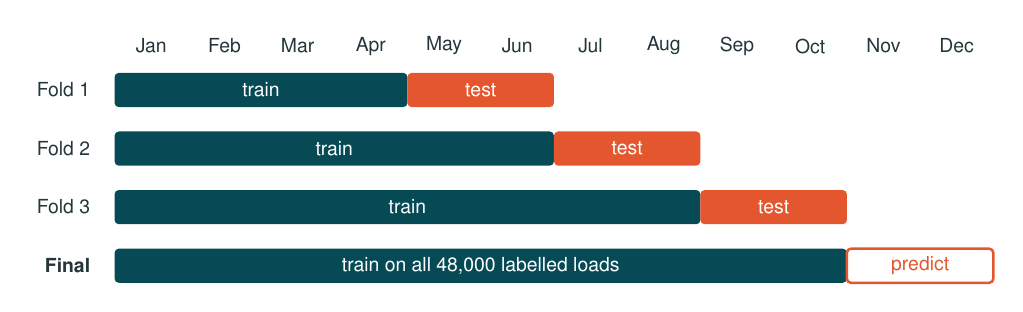
\begin{tikzpicture}[x=0.93cm,y=0.62cm,font=\sans\scriptsize]
  \foreach \m [count=\i from 0] in {Jan,Feb,Mar,Apr,May,Jun,Jul,Aug,Sep,Oct,Nov,Dec}{
    \node[text=ink] at (\i+2.6+0.5,0.9) {\m};}
  \foreach \lab/\tr/\te/\row in {Fold 1/4/2/-0,Fold 2/6/2/-1.2,Fold 3/8/2/-2.4}{
    \node[anchor=east,text=ink] at (2.4,\row) {\lab};
    \fill[teal,rounded corners=1.5pt] (2.6,\row-0.35) rectangle (2.6+\tr,\row+0.35);
    \fill[coral,rounded corners=1.5pt] (2.6+\tr,\row-0.35) rectangle (2.6+\tr+\te,\row+0.35);
    \node[text=white] at (2.6+\tr/2,\row) {train};
    \node[text=white] at (2.6+\tr+\te/2,\row) {test};}
  \node[anchor=east,text=ink] at (2.4,-3.6) {\textbf{Final}};
  \fill[teal,rounded corners=1.5pt] (2.6,-3.95) rectangle (12.6,-3.25);
  \fill[white,draw=coral,line width=0.9pt,rounded corners=1.5pt] (12.6,-3.95) rectangle (14.6,-3.25);
  \node[text=white] at (7.6,-3.6) {train on all \xNTrain{} labelled loads};
  \node[text=coral] at (13.6,-3.6) {predict};
\end{tikzpicture}
\caption{Expanding-window validation. The final fit uses all labelled data to predict the unseen Nov--Dec loads.}
\end{figure}
\newpage

\subsection{Leakage controls and metrics}
\begin{itemize}
  \item Date-level signals (daily median \texttt{market\_index}, mean \texttt{quote\_signal}) are computed from \emph{feature columns only}; the label is never touched.
  \item Model selection and the level-offset window were chosen on the folds above; the final model is refit on all labelled rows.
  \item Because the grading metric is not disclosed, I report MAE, MAPE, median absolute percentage error, and RMSE in dollars.
\end{itemize}

% ================= 3 =================
\section{What the data looks like}
\subsection{Price structure}
Rate is multiplicative in its drivers, so everything is modelled on a log scale. A robust log-linear fit gives a distance
elasticity of about \xElastDist, a Reefer premium of about \xReeferPct\% and a Flatbed premium of about \xFlatbedPct\% over Dry Van.
Rate per mile falls with distance (a short-haul premium), so the relationship is not a pure power law and a non-linear model helps.
Weight, \texttt{market\_index} and \texttt{quote\_signal} have small effects.

\begin{figure}[H]
\centering
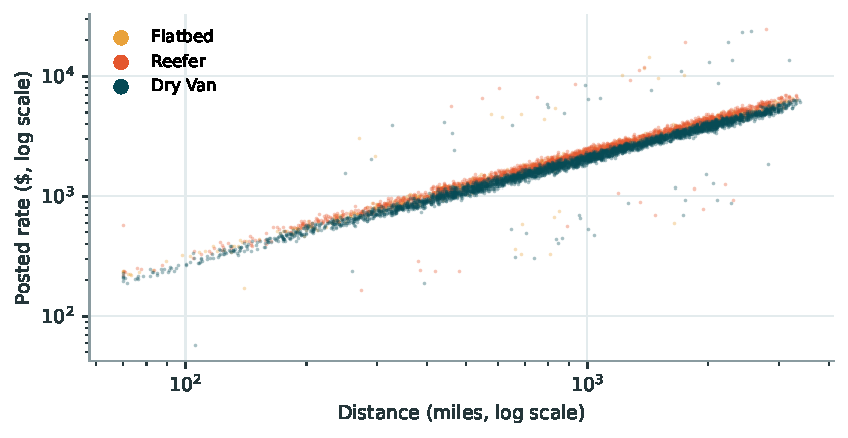
\includegraphics[width=0.8\textwidth]{figures/eda_loglog.pdf}
\caption{Rate versus distance on log axes (7{,}000 sampled loads). The cloud is close to linear, with equipment-specific offsets and a thin band of outliers.}
\end{figure}

\subsection{The market has shifted}
\texttt{market\_index} is a date-level signal (within-day standard deviation $\approx\xMIWithinStd$). Its training range was
\xMITrainMin--\xMITrainMax{} but in the prediction period it is much calmer: \xMIValMin--\xMIValMax{} with mean \xMIValMean.
Tree models cannot extrapolate beyond the training range, but the prediction period sits entirely inside it, so this is a distribution shift rather than an extrapolation problem.

\begin{figure}[H]
\centering
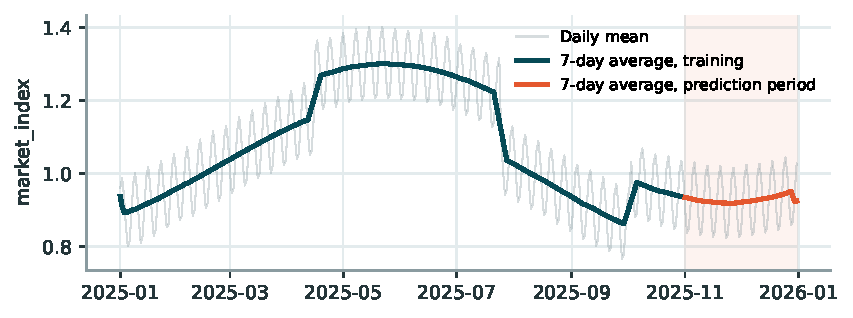
\includegraphics[width=0.86\textwidth]{figures/market_index.pdf}
\caption{Daily mean \texttt{market\_index}. It has a strong weekly cycle on top of a slow trend; the prediction period (shaded) is calmer than the spring--summer peak.}
\end{figure}

% ================= 4 =================
\section{Data-quality issues and how they were handled}
\begin{table}[H]
\centering\small
\begin{tabularx}{\textwidth}{@{}>{\raggedright\arraybackslash}p{3.0cm}>{\raggedright\arraybackslash}X>{\raggedright\arraybackslash}X@{}}
\toprule
\textbf{Issue} & \textbf{Evidence} & \textbf{Handling} \\
\midrule
Negative weights & \xNegWeightTrain{} train / \xNegWeightVal{} prediction rows; magnitudes match the positive distribution (5{,}000--47{,}500\,lb) & Sign errors: use $|w|$ \\
Missing weight & \xMissWeightTrain{} train / \xMissWeightVal{} prediction rows & Training median \\
Missing \texttt{market\_index} & \xMissMITrain{} train / \xMissMIVal{} prediction rows; it is date-level & Median of that date \\
Corrupted labels & \xSpikePct\% of rows are $\times$\xSpikeHiMult{} or $\times$\xSpikeLoMult{} of the expected rate, spread evenly over months, equipment and \texttt{quote\_signal} & Keep rows; robust L1 loss on $\log$ rate \\
Unseen cities & \xNUnseen{} cities in the prediction set absent from training & No city or coordinate features \\
Noisy distance & Floor of \xDistFloor{} miles; same lane varies by a few percent; some rows disagree with coordinates & Use the \texttt{distance} column directly \\
\bottomrule
\end{tabularx}
\caption{Data-quality audit.}
\end{table}

\begin{figure}[H]
\centering
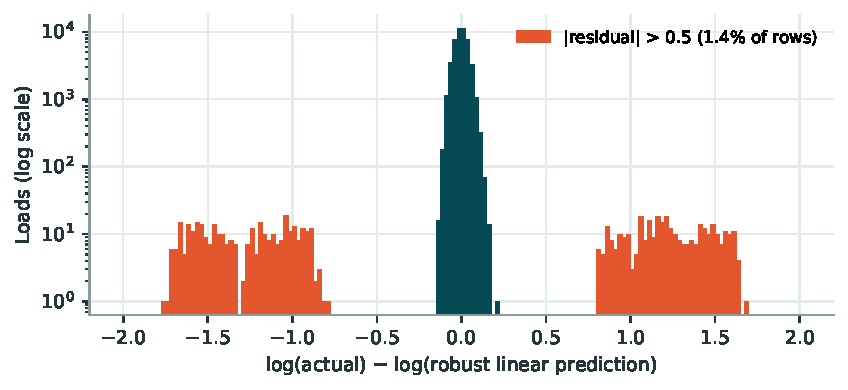
\includegraphics[width=0.86\textwidth]{figures/label_spikes.pdf}
\caption{Residuals of a robust linear fit. The core is tight (about \xCoreSigma\% noise); the coral tails are labels that no feature explains. They would dominate a squared-error objective, which is why the final model uses absolute error.}
\end{figure}

% ================= 5 =================
\Needspace{16\baselineskip}
\section{Modelling}
\subsection{Pipeline}
\begin{figure}[H]
\centering
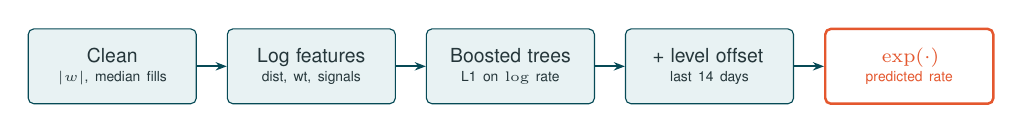
\begin{tikzpicture}[font=\sans\scriptsize,node distance=0.38cm,
  b/.style={draw=teal,fill=lightteal,rounded corners=2pt,minimum height=0.95cm,text width=1.9cm,align=center,text=ink},
  fin/.style={draw=coral,fill=white,rounded corners=2pt,minimum height=0.95cm,text width=1.9cm,align=center,text=coral,line width=0.9pt},
  a/.style={-{Stealth[length=4pt]},teal,line width=0.8pt}]
  \node[b] (a1) {Clean\\[-1pt]{\tiny $|w|$, median fills}};
  \node[b,right=of a1] (a2) {Log features\\[-1pt]{\tiny dist, wt, signals}};
  \node[b,right=of a2] (a3) {Boosted trees\\[-1pt]{\tiny L1 on $\log$ rate}};
  \node[b,right=of a3] (a4) {+ level offset\\[-1pt]{\tiny last 14 days}};
  \node[fin,right=of a4] (a5) {$\exp(\cdot)$\\[-1pt]{\tiny predicted rate}};
  \foreach \i/\j in {a1/a2,a2/a3,a3/a4,a4/a5} \draw[a] (\i)--(\j);
\end{tikzpicture}
\caption{End-to-end pipeline implemented in \texttt{train.py}.}
\end{figure}

\subsection{Features}
Six inputs: $\log$ distance, $\log$ weight, $\log$ \texttt{market\_index}, $\log$ \texttt{quote\_signal}, and Reefer and Flatbed flags.
Day-of-week, day-of-year, coordinate differences and city identity were tested in rolling validation and rejected: day-of-week and coordinates were neutral to slightly worse,
and day-of-year was about 6\% worse in MAE because one year of data cannot identify seasonality.

\subsection{Model choice}
\begin{itemize}
  \item \textbf{Baseline:} Huber regression on $\log$ rate. Robust and interpretable, but it misses the non-linear distance curve and interactions.
  \item \textbf{Final:} \texttt{HistGradientBoostingRegressor} with \texttt{loss="absolute\_error"} on $\log$ rate. Trees capture the short-haul premium; the L1 loss
        predicts a conditional median, so corrupted labels barely move it. In development, squared-error loss was roughly 8\% worse in MAE.
  \item \textbf{Early stopping is disabled} and the seed is fixed so results are reproducible across machines.
\end{itemize}

\subsection{Recent-level correction}
Residuals show a slow price-level drift (monthly median residual between about $-3\%$ and $+3\%$) that \texttt{market\_index} does not explain.
After fitting, I take the median residual over the last 14 days before the cutoff and add it to every prediction.
For the final model this offset is \xOffset. The code is short:

\begin{codebox}
\begin{lstlisting}[style=py]
def level_offset(model, X, y, dates, cutoff):
    start = cutoff - pd.Timedelta(days=LEVEL_WINDOW_DAYS)
    recent = (dates >= start) & (dates < cutoff)
    resid = y[recent] - model.predict(X.loc[recent, FEATURES])
    return float(np.median(resid))
\end{lstlisting}
\end{codebox}

% ================= 6 =================
\section{Results}
\begin{table}[H]
\centering\small
\begin{tabular}{@{}lrrrr@{}}
\toprule
\textbf{Model (mean of 3 folds)} & \textbf{MAE (\$)} & \textbf{MAPE (\%)} & \textbf{MedAPE (\%)} & \textbf{RMSE (\$)} \\
\midrule
Huber log-linear (baseline) & 138.9 & 6.03 & 3.42 & 639.9 \\
Gradient boosting, L1 loss & 125.4 & 5.44 & 2.47 & 634.9 \\
\textbf{Boosting + level offset (final)} & \textbf{118.4} & \textbf{5.17} & \textbf{2.15} & \textbf{632.5}
\\
\bottomrule
\end{tabular}
\caption{Forward-in-time validation. RMSE is dominated by corrupted labels and barely separates the models, so decisions rely on MAE and median error.}
\end{table}

The final model beats the baseline by \xGainMAE\% on MAE and \xGainMed\% on median percentage error. The level offset alone is worth \$\xOffsetGainMAE{} of MAE.

\begin{figure}[!htbp]
\centering
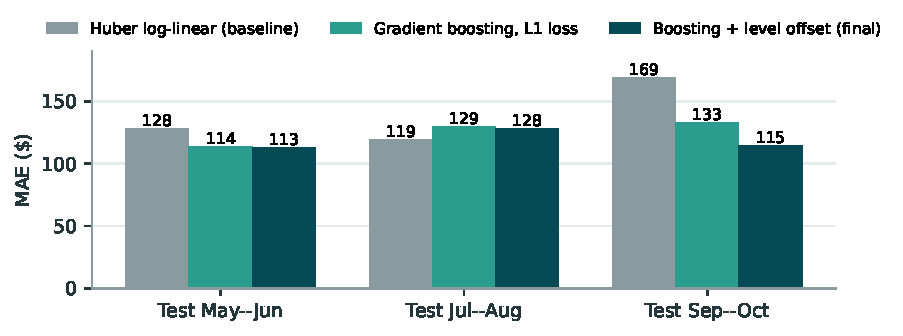
\includegraphics[width=0.74\textwidth]{figures/cv_mae.pdf}
\caption{MAE by fold. The boosted model wins in two of three folds; in Jul--Aug a baseline fit on Jan--Jun happened to track that window slightly better.}
\end{figure}

\begin{table}[H]
\centering\small
\begin{tabular}{@{}lrrr@{}}
\toprule
\textbf{Test window} & \textbf{Huber} & \textbf{Boosting} & \textbf{Final} \\
\midrule
May--Jun & 127.8 & 113.6 & 112.8 \\
Jul--Aug & 119.4 & 129.5 & 127.9 \\
Sep--Oct & 169.4 & 133.1 & 114.6
\\
\bottomrule
\end{tabular}
\caption{MAE (\$) per fold.}
\end{table}

\subsection{Diagnostics on the Sep--Oct fold}
\begin{figure}[H]
\centering
\begin{subfigure}{0.48\textwidth}\centering
  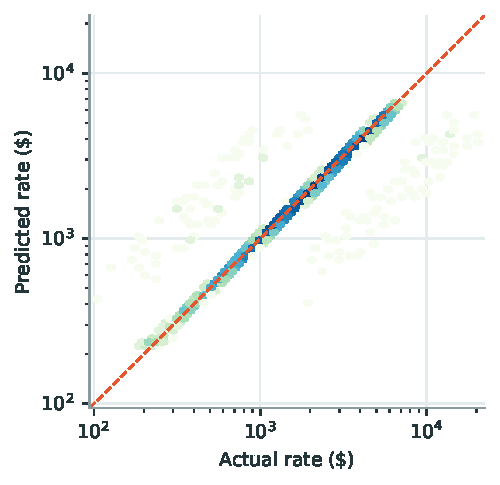
\includegraphics[width=\linewidth]{figures/pred_vs_actual.pdf}
  \caption{Predicted versus actual (log axes). Points hug the diagonal; the off-diagonal arms are the corrupted labels.}
\end{subfigure}\hfill
\begin{subfigure}{0.48\textwidth}\centering
  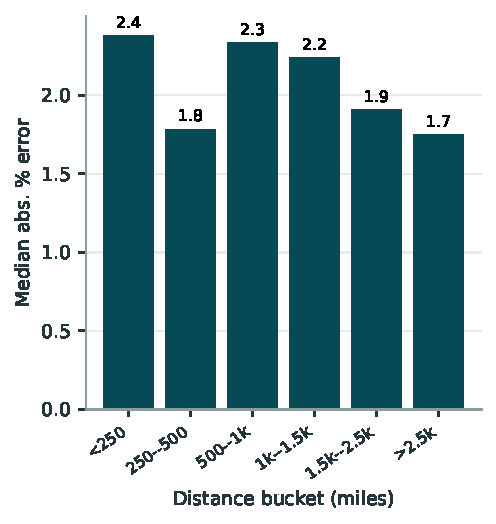
\includegraphics[width=\linewidth]{figures/error_by_distance.pdf}
  \caption{Median error by distance bucket: from \xMedAPELong\% on the longest hauls to about \xMedAPEShort\% on the shortest.}
\end{subfigure}
\caption{Hold-out diagnostics. Overall median error on this fold is \xMedAPEFold\%.}
\end{figure}

\begin{figure}[H]
\centering
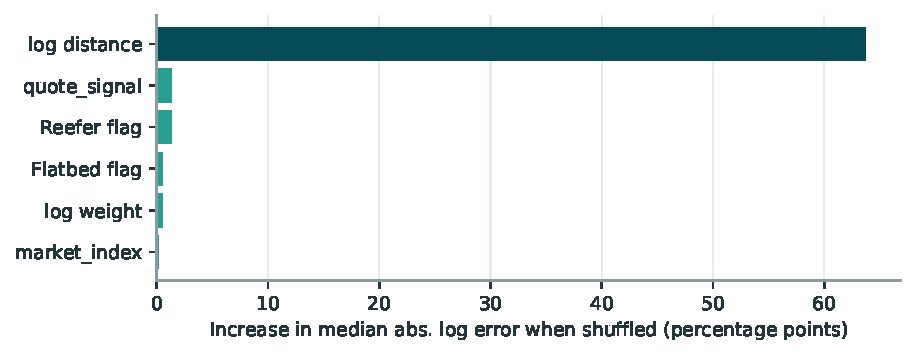
\includegraphics[width=0.78\textwidth]{figures/importance.pdf}
\caption{Permutation importance on the hold-out fold: shuffling \xTopFeature{} hurts far more than shuffling any other input. Market signals and equipment add small refinements, in line with the weak correlations seen in exploration.}
\end{figure}

% ================= 7 =================
\Needspace{14\baselineskip}
\section{Fixed December chart}
The chart was produced by the provided \texttt{score.py}. Inputs are fixed (Lexington $\rightarrow$ Fort Wayne, 360 miles, Dry Van, 32{,}000\,lb) and only the date varies.
These rows carry no \texttt{market\_index} or \texttt{quote\_signal}, so each date uses the daily median of those signals from the December prediction loads (feature columns only).

\begin{figure}[H]
\centering
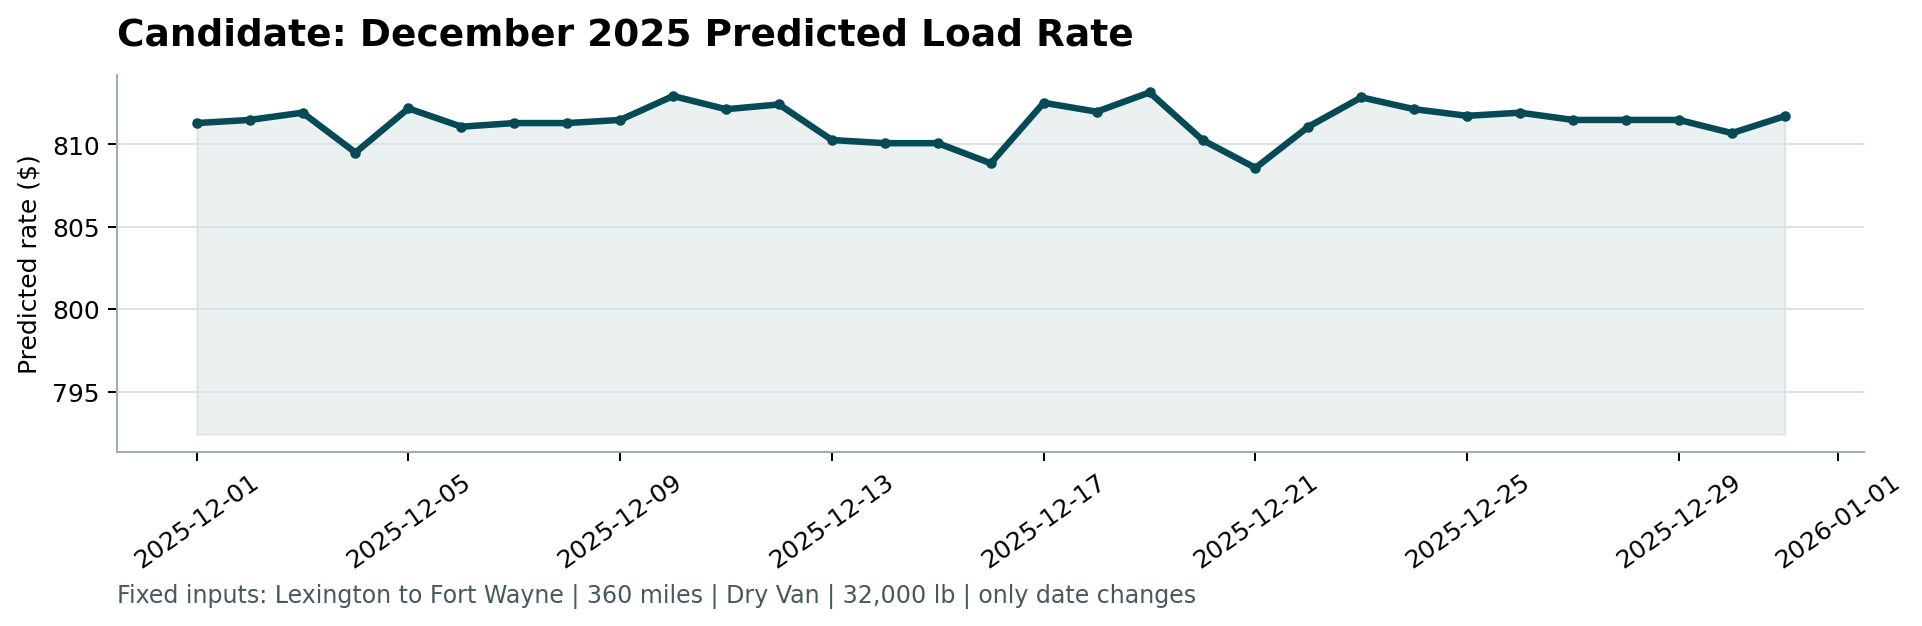
\includegraphics[width=0.84\textwidth]{figures/candidate_december.png}
\caption{Predicted December 2025 rate for the fixed lane.}
\end{figure}

\begin{callout}[title=How to read it]
Predictions range from \$\xDecMin{} to \$\xDecMax{} (mean \$\xDecMean), a total spread of only \xDecSpreadPct\%.
The scorer zooms the vertical axis, which makes day-to-day moves look large. Within a month the only date-varying inputs are the two market signals,
which the model finds to be weak drivers, so a flat profile is the honest forecast. I do not claim a holiday effect:
the training data contains no December from which to learn one.
\end{callout}

% ================= 8 =================
\section{Limitations and next steps}
\begin{itemize}
  \item \textbf{Ten months of history} cannot reveal annual seasonality. With several years, month and holiday features would become learnable.
  \item \textbf{Level drift is carried forward, not forecast.} If November--December rates move away from the October level, the offset will not anticipate it.
  \item \textbf{Small tuning set.} The 14-day window and the offset benefit were selected on four folds from one year; treat the gain as moderate evidence.
  \item \textbf{Corrupted labels} in any hidden evaluation set will inflate RMSE for every model, including this one.
  \item \textbf{Next steps:} quantile models for prediction intervals, a lane-level target encoding that gracefully handles unseen cities, and an explicit detector for corrupted labels.
\end{itemize}

\Needspace{9\baselineskip}
\section*{Reproducing the results}
\begin{codebox}
\begin{lstlisting}[style=py,language={},basicstyle=\ttfamily\scriptsize\color{ink}]
python -m pip install -r requirements.txt
python train.py
python score.py --predictions validation_predictions.csv --december-predictions data/december_chart_inputs.csv
python report/make_assets.py      # figures and numbers for this report
\end{lstlisting}
\end{codebox}

\end{document}
